\chapter{Introducción específica} % Main chapter title

\label{Chapter2}

%----------------------------------------------------------------------------------------
%	SECTION 1
%----------------------------------------------------------------------------------------
En este capítulo se presentan las distintas tecnologías y metodologías disponibles para la implementación del prototipo de robot móvil. Se describen los dispositivos y arquitecturas más significativos que permitieron alcanzar los requerimientos planteados.

\section{Módulos y dispositivos de hardware}

En esta sección se describen los Módulos y dispositivos de hardware que componen el prototipo robot desarrollado


\subsection{Placa de microprocesamiento}
Se utilizó  la placa de desarrollo EDUCIAA-NXP \citep{EDUCIAA} ya que la misma se usa para la ejercitación en varias asignaturas de la carrera de postgrado. En la figura \ref{fig:EDUCIAANXP} se observa una imagen de la EDU-CIAA-NXP, una versión de bajo costo de la CIAA-NXP, pensada para la enseñanza universitaria, terciaria y secundaria. 

\begin{figure}[htpb]
	\centering
	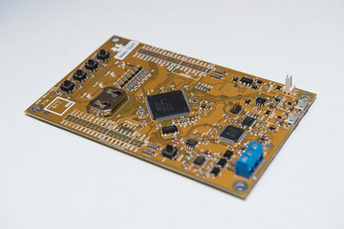
\includegraphics[width=\textwidth]{./Figures/EDUCIAANXP.jpg}
	\caption{Placa de desarrollo EDUCIAA-NXP\protect\footnotemark.}
	\label{fig:EDUCIAANXP}
\end{figure}
\footnotetext{Imagen tomada de \url{http://www.proyecto-ciaa.com.ar}}

\pagebreak

En la figura \ref{fig:Bloques} puede verse un diagrama en bloques general de la placa. 

\begin{figure}[htpb]
	\centering
	\includegraphics[width=9cm]{./Figures/Bloques.jpg}
	\caption{Diagrama en bloques de la EDUCIAA-NXP.\protect\footnotemark.}
	\label{fig:Bloques}
\end{figure}
\footnotetext{Imagen tomada de \url{http://www.proyecto-ciaa.com.ar}}

El  microcontrolador utilizado por la EDU-CIAA es el LPC4337 (dual core ARM Cortex-M4F y Cortex-M0). Los recursos más significativos que se utilizaron de la placa fueron: 


\begin{itemize}
	\item GPIO (General Purpose Input/Output, Entrada/Salida de Propósito General)
	\item PWM (Pulse Width Modulation, modulación por ancho de pulso).
	\item UART (Universal Asynchronous Receiver-Transmitter, Transmisor-Receptor Asíncrono Universal).
	\item Temporizadores.
\end{itemize}


\subsection{Driver de motores}

Se utilizó un módulo para el accionamiento de motores \citep{Driver}. En la figura \ref{fig:Driver} se puede observar una imagen de la placa 
El módulo está basado en el circuito integrado L298N \citep{L298} y permite controlar dos motores de corriente continua de manera simultánea e independiente.  Sus características principales son:

\begin{itemize}
	\item Tensión mínima: 5 V.
	\item Tensión máxima: 35 V.
	\item Corriente máxima: 2 A.
	\item Tensión de nivel lógico: 5 V.
	\item Potencia máxima 25 W.
	\item Medidas: 43 x 43 x 24 mm.
\end{itemize}
\pagebreak

\begin{figure}[h]
	\centering
	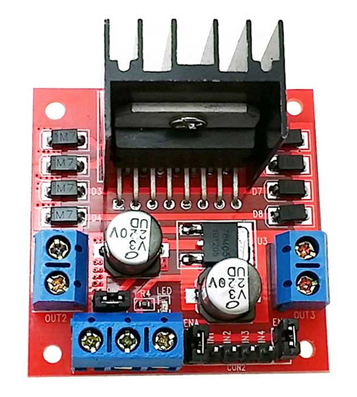
\includegraphics[width=5cm]{./Figures/L298N.png}
	\caption{Driver de motores.\protect\footnotemark.}
	\label{fig:Driver}
\end{figure}
\footnotetext{Imagen tomada de \url{http://robots-argentina.com.ar}}


La placa tiene la opción de habilitar o no el regulador LM7805 integrado para alimentar la parte lógica. En la figura \ref{fig:Esquema} se observa el diagrama esquemático del módulo.


\begin{figure}[h]
	\centering
	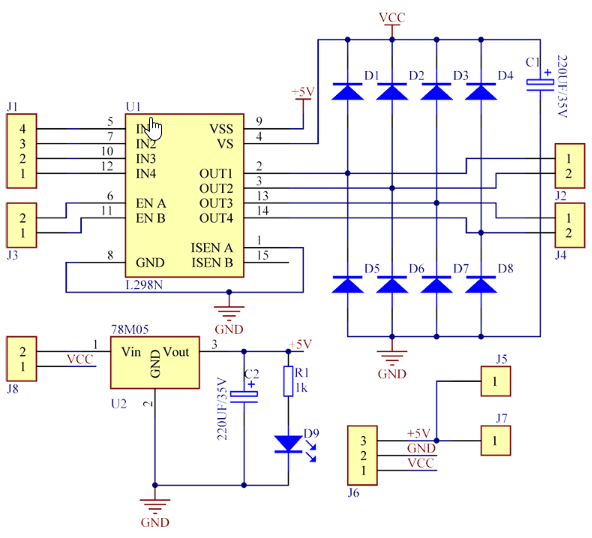
\includegraphics[width=12cm]{./Figures/Modulo.png}
	\caption{diagrama esquemático del módulo.\protect\footnotemark.}
	\label{fig:Esquema}
\end{figure}
\footnotetext{Imagen tomada de \url{http://robots-argentina.com.ar}}




\subsection{Módulo sensor de infrarrojos}

Se utilizaron dos módulos sensores de proximidad por infrarrojos IR FC-51 \citep{IR} para la detección de obstáculos por parte del robot. Estos módulos están compuestos por  un emisor de luz infrarroja (IR)  y un receptor que detecta su reflejo en  las superficies contra las que se enfrenta, de modo que presentan una señal en  presencia de cualquier obstáculo en su parte frontal. Un potenciómetro permite ajustar el rango de detección. 

El sensor presenta una respuesta estable incluso con luz ambiente o en completa oscuridad. En la figura \ref{fig:moduloIR} se observa una imagen del sensor de infrarrojos.

\begin{figure}[h]
	\centering
	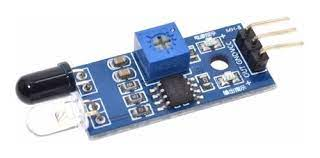
\includegraphics[width=8cm]{./Figures/moduloIR.jpg}
	\caption{Módulo sensor de infrarrojos \protect\footnotemark.}
	\label{fig:moduloIR}
\end{figure}
\footnotetext{Imagen tomada de \url{http://robots-argentina.com.ar}}



En la figura \ref{fig:IRschem} se muestra el circuito esquemático  del sensor de Infrarrojos

\begin{figure}[h]
	\centering
	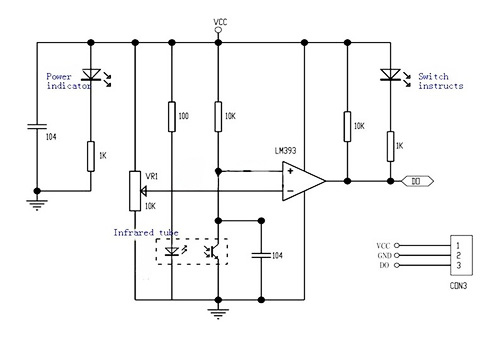
\includegraphics[width=14cm]{./Figures/IRschem.jpg}
	\caption{Esquema del módulo sensor de Infrarrojos .\protect\footnotemark.}
	\label{fig:IRschem}
\end{figure}
\footnotetext{Imagen tomada de \url{http://robots-argentina.com.ar}}
\pagebreak

Las características del módulo son:
\begin{itemize}
	\item Ángulo de cobertura: 35°.
	\item Tensión de funcionamiento: 3 V – 6 V.
	\item Rango de detección: 2 cm – 30 cm (ajustable con el potenciómetro).
	\item Tamaño: 4,5 cm x 1,4 cm x 0,7 cm. 
	\item Discriminación: la salida toma nivel lógico bajo cuando se detecta un obstáculo (reflexión).
\end{itemize}



\subsection{Baterías}

En función del consumo y la intensión de no dedicar mayor espacio a las celdas de alimentación, se emplearon dos baterías de Ion-litio tipo 18650. Una de las ventajas de las Ion-litio es que permiten ser recargadas con una media de entre 600 a 1000 veces sin que se estropeen ni pierdan efectividad \citep{18650}. La capacidad de estas baterías varían de un modelo a otro pero suelen estar comprendidas entre los 2100 mAH y los 4000mAH. Su tensión nominal es de 3,7 V (hasta 4,2 V en vacío).

Las baterías van conectadas en serie para lograr una tensión de 7,4 V acorde a la alimentación de los motores y con un margen superior necesario para el correcto funcionamiento del regulador de tensión de 5 V del módulo de accionamiento de motores. 
Las baterías se insertaron en un portapilas comercial. En la figura \ref{fig:portapila} se muestra las dos baterías 18650 ya instaladas en su portapila.


\begin{figure}[h]
	\centering
	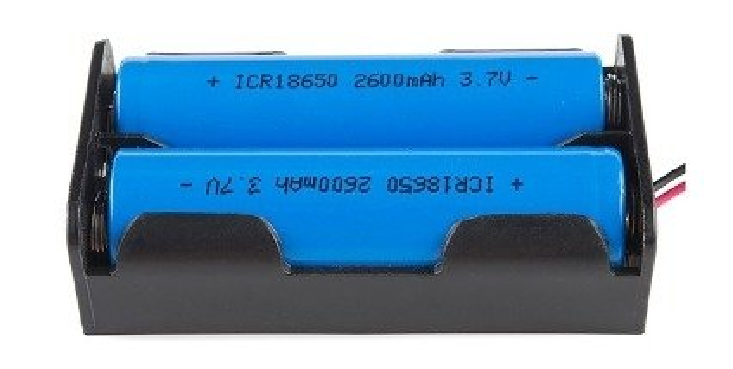
\includegraphics[width=10cm]{./Figures/portapilas.PNG}
	\caption{Las dos baterías 18650 en su portapila .}
	\label{fig:portapila}
\end{figure}


\subsection{Módulo de comunicaciones Bluetooth}

Se utilizó el módulo Bluetooth HC-05 para la comunicación comunicaciones con el robot \citep{HC05}. El mismo ya había sido utilizado en  prácticas de la asignatura “Protocolos de comunicaciones en sistemas embebidos”, conectado al puerto serie de la EDU-CIAA. Todos los parámetros del módulo se pueden configurar mediante comandos AT. 

En la figura \ref{fig:moduloHC05} se observa el módulo HC-05.


\begin{figure}[h]
	\centering
	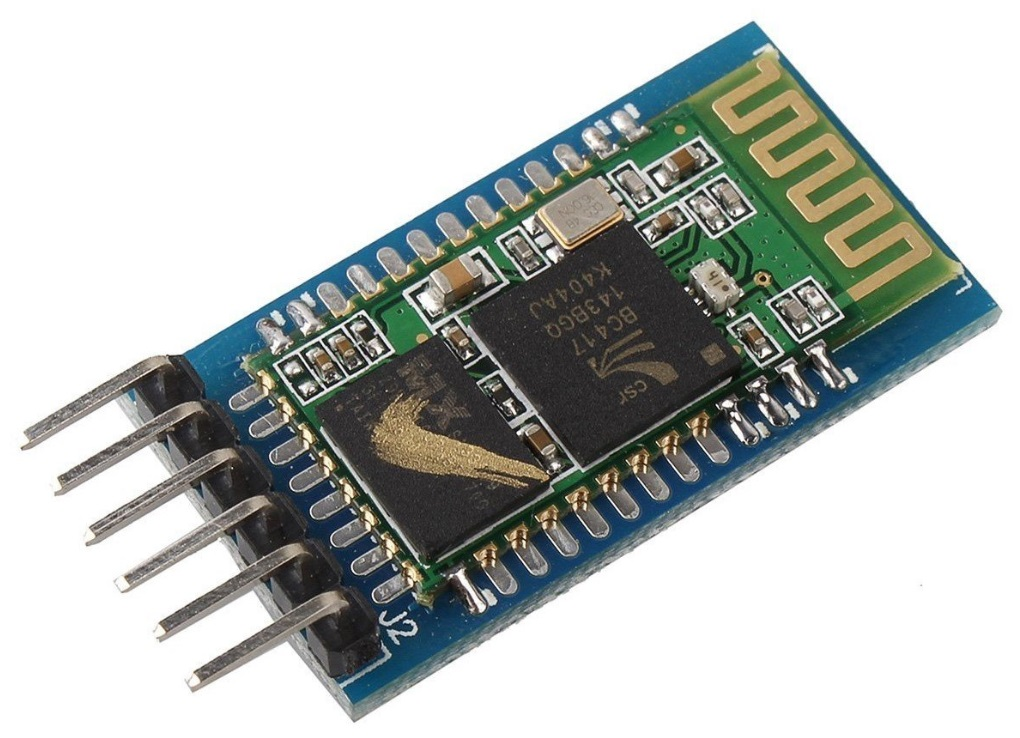
\includegraphics[width=8cm]{./Figures/HC05.jpeg}
	\caption{Módulo Bluetooth HC-05 .\protect\footnotemark.}
	\label{fig:moduloHC05}
\end{figure}
\footnotetext{Imagen tomada de \url{https://maker.pro/custom/tutorial/hc-05-bluetooth-transceiver-module-datasheet-highlights}}



Las características del módulo son:
\begin{itemize}
	\item Voltaje de operación: 3.6 V - 6 V DC.
	\item Consumo corriente: 50 mA.
	\item Bluetooth: V2.0+EDR.
	\item Frecuencia: Banda ISM 2.4 GHz.
	\item Modulación: GFSK(Gaussian Frequency Shift Keying)
	\item Potencia de transmisión: 4 dBm, Class 2.
	\item Sensibilidad: -84dBm a 0.1% BER.
	\item Alcance 10 m.
	\item Tamaño: 3,7 cm x 1,6 cm.
\end{itemize}




%----------------------------------------------------------------------------------------
%	SECTION 2
%-----------------------------------------------------------------
\section{Requerimientos}

En esta sección se enumeran los requerimientos planteados en la planificación inicial del proyecto.  Los  requerimientos se han dividido en funcionales y no funcionales.

\label{sec:requerimientos}

\begin{enumerate}
\item Requerimientos funcionales
	\begin{enumerate}
	\item Capacidad de locomoción.  El robot debe ser capaz de desplazarse por medio de ruedas motorizadas, a través de superficies planas.
	\item Capacidad de percepción. El robot debe ser capaz de detectar y obtener información del medio. 
	\item Capacidad de comunicación inalámbrica.
	\item El robot deberá funcionar con alimentación a batería recargable.
	\item El proyecto debe ser extensible a una posible herramienta de enseñanza e investigación

	\end{enumerate}
\item Requerimientos no funcionales
	\begin{enumerate}
	\item El robot no debe resultar peligroso para el ambiente o las personas con las que podría interactuar.
	\item El diseño del robot debe respetar regulaciones en cuanto a radiación en el espectro ultravioleta.
	\item Se utilizarán componentes electrónicos disponibles comercialmente en Argentina.
	\end{enumerate}
\end{enumerate}

\section{Planificación}

El trabajo se organizó para ser terminado en el mes de junio de 2021 con una dedicación aproximada de 600 horas en total. Con el fin de organizar y dar seguimiento a las actividades requeridas y poder identificar los desvíos en los tiempos de ejecución programados, se cuantificaron los tiempos de las diversas tareas mediante el diagrama de Gantt, que se observa en las figuras \ref{fig:gantt1} y \ref{fig:gantt2}.


\begin{figure}[htpb]
\centering 
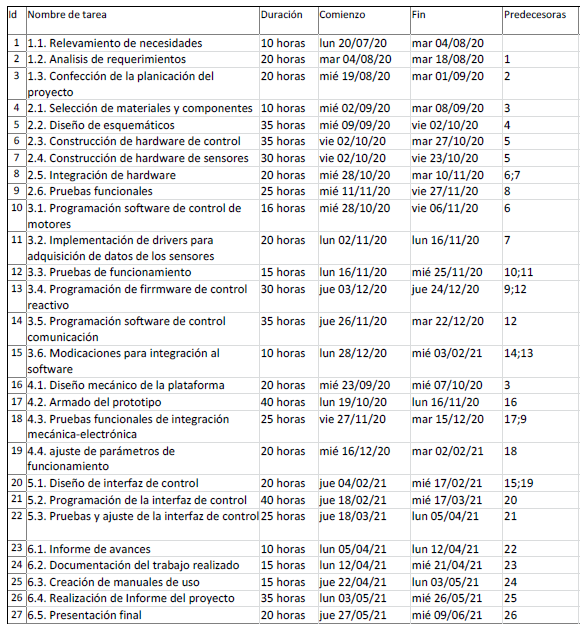
\includegraphics[width=\textwidth]{./Figures/gantttabla.PNG}
\caption{Tabla de tareas de Gantt}
\label{fig:gantt1}
\end{figure}

\begin{figure}[htpb]
\centering 
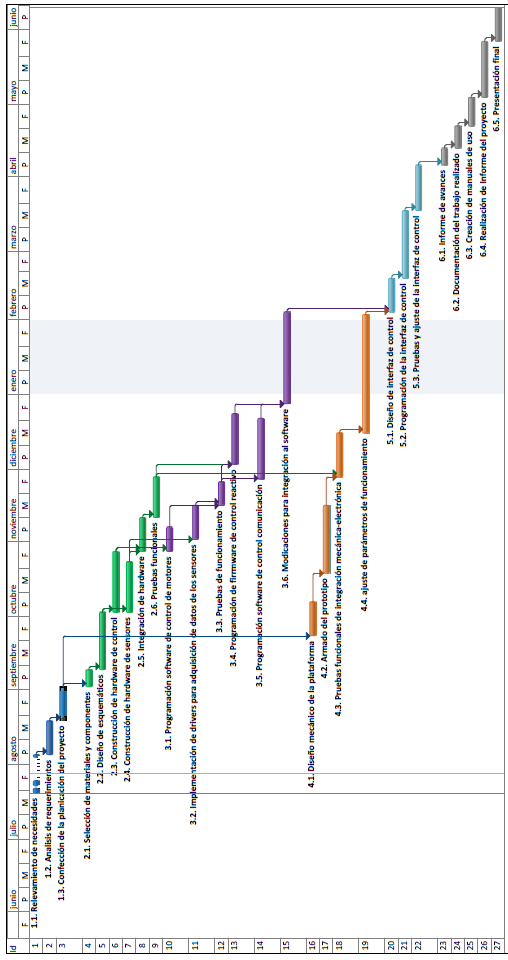
\includegraphics[width=\textwidth]{./Figures/Gantt.PNG}
\caption{Diagrama de Gantt}
\label{fig:gantt2}
\end{figure}

\pagebreak

Se confeccionó también un diagrama de Activity on Node, con la finalidad de resaltar las tareas cuyos retrasos podrían resultar críticos para la concreción del trabajo. En rojo se indica el camino crítico, como puede apreciarse en la figura \ref{fig:AoN}

\begin{figure}[htpb]
\centering 
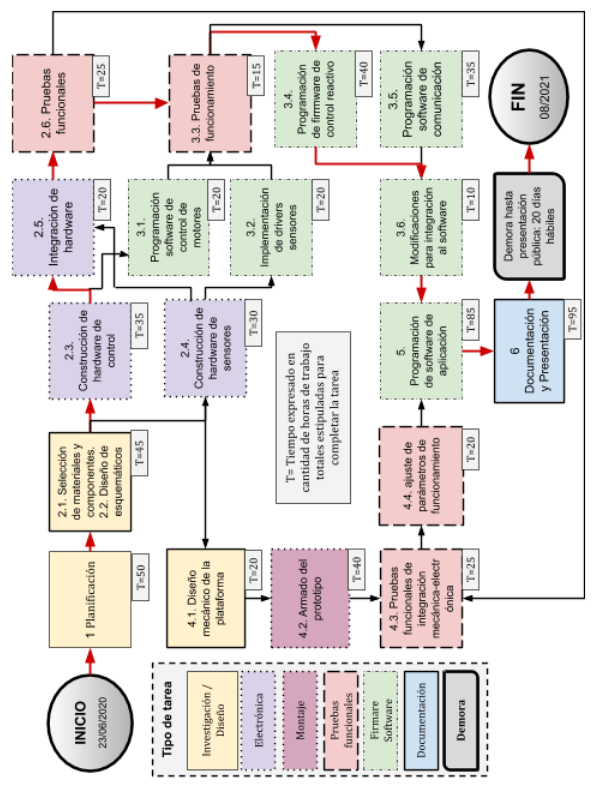
\includegraphics[width=\textwidth]{./Figures/AoN.png}
\caption{Diagrama en \textit{Activity on Node}}
\label{fig:AoN}
\end{figure}


A partir de este análisis está organizado el trabajo que se presenta en los próximos capítulos.

